\documentclass[twocolumn]{article}
\usepackage{graphicx}
\usepackage{multicol}

\begin{document}

\begin{center}\Large\textbf{Raw Results}\end{center}

\section{First Runs}

\subsection{Cls}
These are the results from tests run for the poster competition. As you can see in figure \ref{first_cl}, the distributed version of the algorithm finds values that match expectations. The input data is generated from synfast with \emph{Nside32} and one twelfth of the sky is fed into each run. This explains the higher variation in the low bands. This is similar to another graph generated from the original shared version.


\begin{figure}
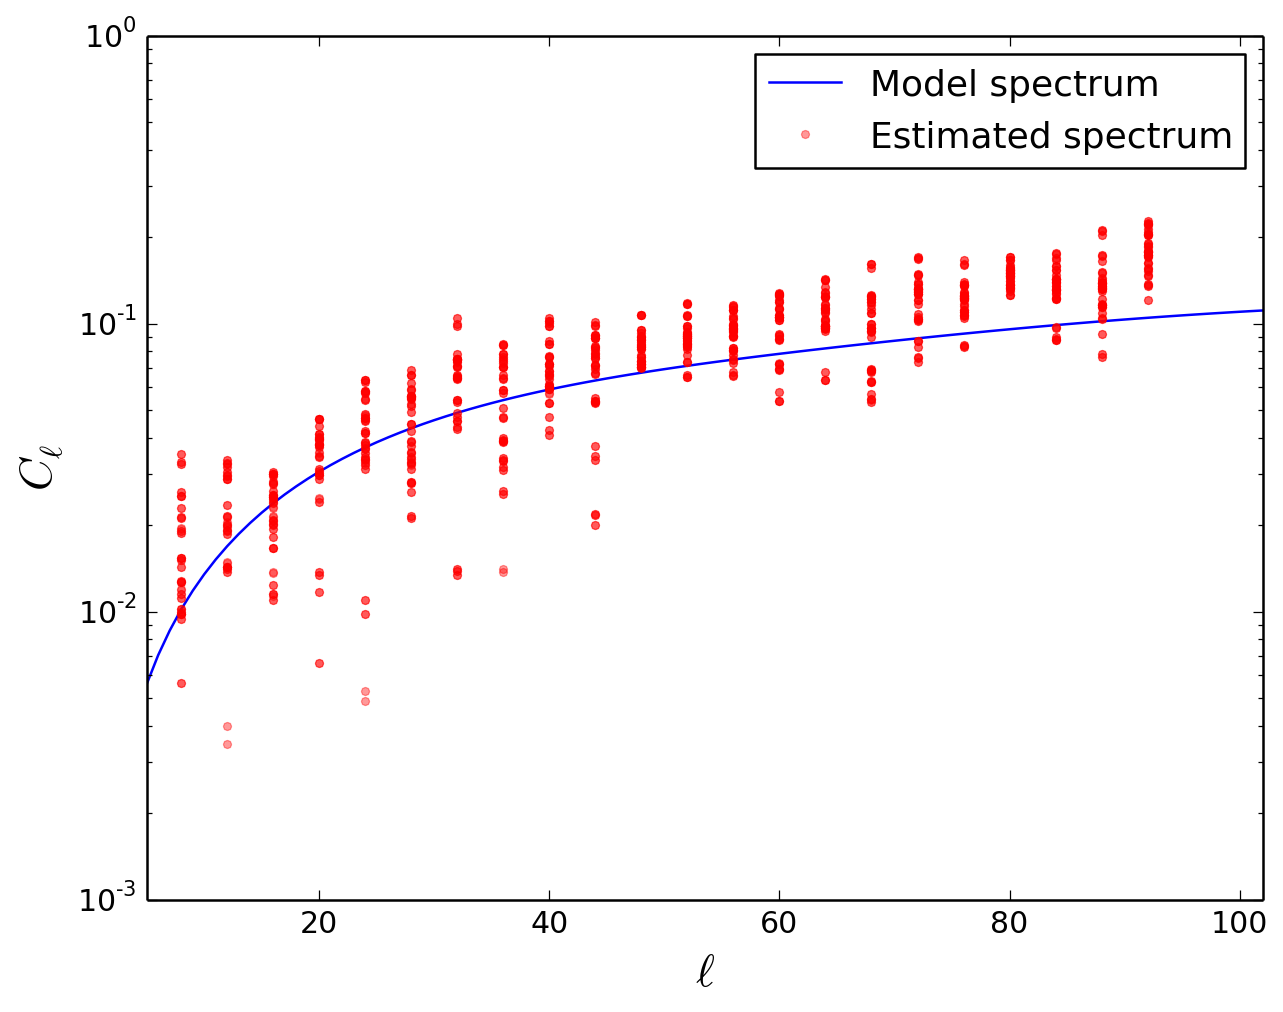
\includegraphics[width=0.9\columnwidth]{figures/cl}
\caption{Cls without KL compression}
\label{first_cl}
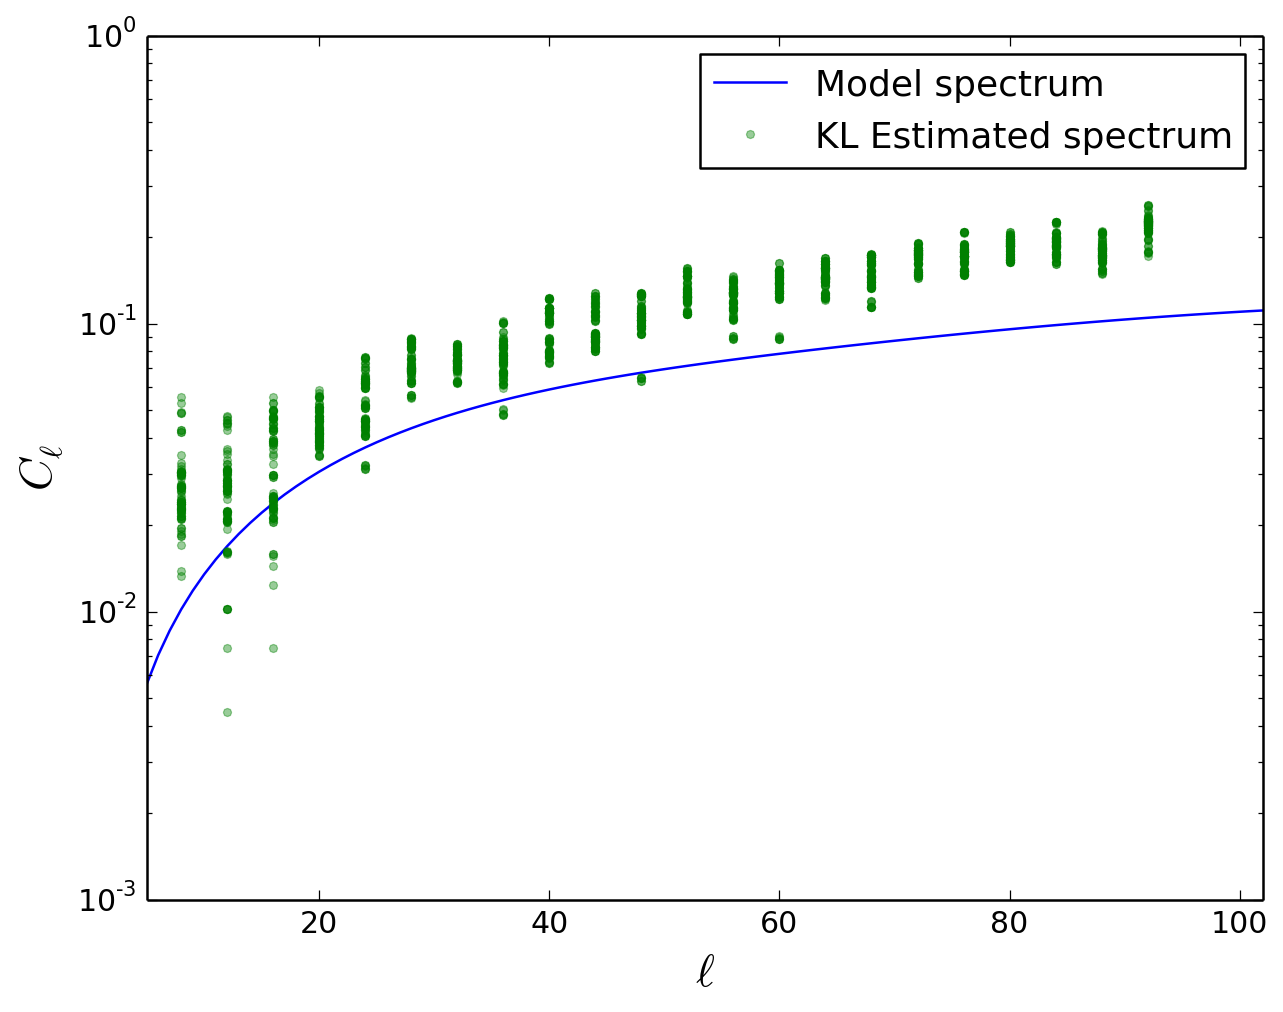
\includegraphics[width=0.9\columnwidth]{figures/kl_cl}
\caption{Cls with KL compression}
\label{first_kl_cl}
\end{figure}

After fixing bugs with KL compression it was possible to do runs to compare the results. In figure \ref{first_kl_cl}, the results do match with the expected line, but with a positive bais. Further investigation is needed to understand the source and nature of the bias.

With the distributed code, it is worth noting that in both runs we were also getting some negative points. This was less the case with KL compression.

\subsection{Time and Memory}

\end{document}